\paragraph{}
IGES\cite{IGES1983} files are used as the bridge between engineering design and numerical analysis.
As a standard file format in engineering design industry, it is supported by almost all design softwares all over the world.
Consequently, by utilizing it we are able to minimize the human effort on mesh generation.

\subsection{Parse geometry in IGES file}
\paragraph{}
The IGES file (explained in detail in \ref{lr_sc:iges}) provides all information that describe the input geometry.
Abstract structure of the IGES file that describe a 2D geometry can be regarded as a simple curve-surface structure.
In other words, it defines the input geometry as certain number of surfaces with different colors.
Different colors represented different material properties in engineering practice.
Each surface contains a list of curve index which is corresponding to the curve information described in IGES file.

\paragraph{}
When IGES file is feed into the programme, each line in the directory entry will be parsed entity by entity.
Parameter in directory entry describe the type and reference to other useful values for the entity.
An entity may reference to one or many entities in directory entry.
Detail of the specification of each entity is explained in \cite{Nasr2007} in detail.

%=====================================================================================================================%
\subsection{Output to mesh generator}
\paragraph{}
The output file that the mesh generator read in will be a shorter summary of the input geometry.
Boundary representation will be kept as the data structure to describe the input geometry.
However, some fields apart from curve and surface will be added.
In the output file, geometry description will be organized as key points, polylines and surfaces.
The key points define the coordinate of all points and polylines are used to represented all curves including NURBS curves for simplification.
NURBS curves can be used directly by the mesh generator as well in \ref{qt_sc:nurbs} but it is found the computational cost in calculation of distance between points to NURBS curves surpass the merits of using it directly.
The exact geometry can be retained by projected the nodes on the boundary back to the origin NURBS curves at the end.

\paragraph{}
Represent a straight line with polyline will not be a problem, first and the last points will be enough to exact representation.
However, that is not the case for curves where curvature is not always zero.
Although using more points must increase the quality of polyline representation, computational cost in the mesh generation when calculating the distance increases at the same time.
Yet, selecting few points that result in a bad polyline representation leads to a poor quality mesh.
Elements may be twisted after the nodes on the boundary are projected to the origin curves.
As a consequence, a quantified index that can control the number and the position of the vertices on the polyline is necessary.

%=====================================================================================================================%
\subsection{Discretization of circular arc}
\paragraph{}
Chord ratio can be a good indicator for circular arc.
The arc length to chord length ratio $\frac{a}{L}$ illustrated in fig.~\ref{qt_fig:iges_chord_ratio} can be expressed in angle $\alpha$ as:
    \begin{equation}
        \frac{a}{L} = \frac{
            \sqrt{2-2\cos\alpha}
        }{\alpha}
        = \frac{
            2\sin\frac{\alpha}{2}
        }{\alpha}
    \end{equation}

The maximum angle $\alpha$ satisfy arc length to chord length ratio $\frac{a}{L} > 1-\epsilon$ with $
    \sin\frac{\alpha}{2} = 1 - \frac{x^3}{6} + O(x^7)
$ can be derived as:
    \begin{equation}
        \alpha < \sqrt{24 \epsilon}
    \end{equation}

    \begin{figure}[h!]
        \centering
        \scalebox{1.2}{
            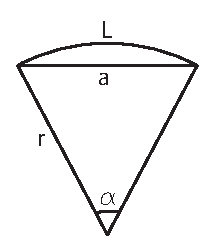
\includegraphics{quadtree/images/iges_chord_ratio.eps}
        }
        \caption{Chord length for circular arc}
        \label{qt_fig:iges_chord_ratio}
    \end{figure}

%=====================================================================================================================%
\subsection{Discretization of NURBS curves}
\paragraph{}
For NURBS curve there is no closed form chord ratio that can be utilized.
However, similar idea can be applied numerically.
The NURBS curves are first divided into serval smaller ones based on the knot vector.  % may be explained in detail
Since the order of each sub-divided NURBS curve used in engineering softwares are predominantly lower or equal to three, the sub-curves then can be divided into two classes, convex curves or concave curve with an inflection point as shown in fig.~\ref{qt_fig:iges_chord_ratio_nurbs}.
    \begin{figure}
        \begin{subfigure}[b]{0.5\linewidth}
            \centering
            \scalebox{0.5}{
                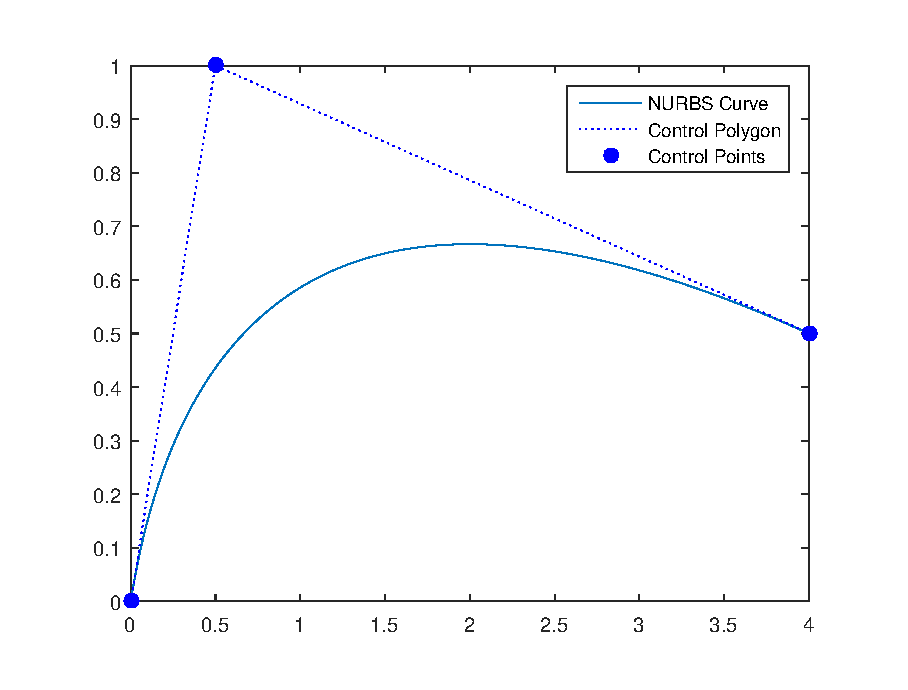
\includegraphics{quadtree/images/iges_chord_ratio_nurbs_convex.eps}
            }
            \caption{Convex}
        \end{subfigure}
        \begin{subfigure}[b]{0.5\linewidth}
            \centering
            \scalebox{0.5}{
                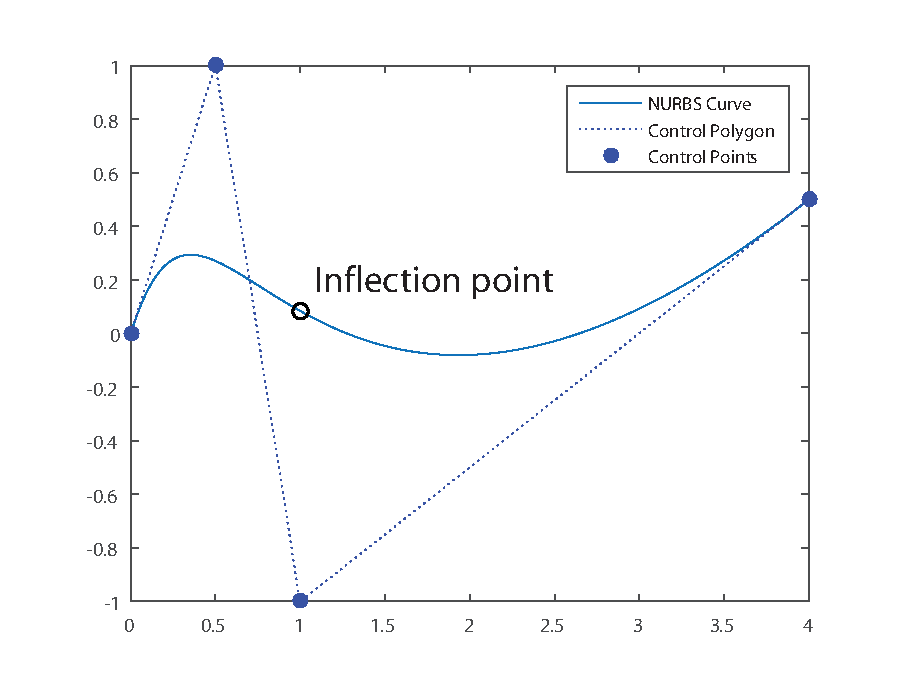
\includegraphics{quadtree/images/iges_chord_ratio_nurbs_concave.eps}
            }
            \caption{Concave with an inflection point}
        \end{subfigure}
    \caption{Type of sub-devided NURBS curves: convex and concave with an inflection point}
    \label{qt_fig:iges_chord_ratio_nurbs}
    \end{figure}

In order to determine the target NURBS curve is convex or concave, a cross product to assess whether the control net will be conducted.
Assuming the target sub-divided NURBS curve is cubic, there will be four control points $P_1,P_2,P_3$ and $P_4$.
If signs of $cross(\overrightarrow{P_1P_2},\overrightarrow{P_2P_3})$ and $cross(\overrightarrow{P_1P_2},\overrightarrow{P_2P_3})$ are the same, then the curve is convex. Otherwise it will be concave.

%=====================================================================================================================%
\subsubsection{Convex curves}
\label{qt_ssc:convex_curves}
\paragraph{}
Start with the simple case, in the situation illustrated in fig.~\ref{qt_fig:iges_chord_split_convex_sum} where line $C(u_0)C(u_n)$ and the NURBS curve form a convex set, we are looking for a point $C(u_m)$ on the curve so that $C'(u_m)$ is parallel to $\overrightarrow{C(u_0)C(u_n)}$
    \begin{figure}[h!]
        \centering
        \scalebox{0.8}{
            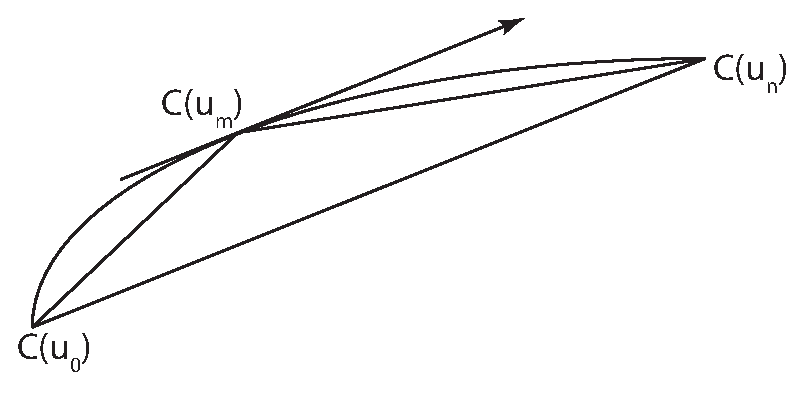
\includegraphics{quadtree/images/iges_chord_split_convex_sum.eps}
        }
        \caption{Discretization for convex NURBS curve}
        \label{qt_fig:iges_chord_split_convex_sum}
    \end{figure}

The target is then split one NURBS curve segment into two.
If any arc length to chord length ratio of these two ratio is below the tolerance given, the splitting will be processed recursively.
Based on the properties of the convex set, there is one and only one parameter $u_m$ that satisfy the condition.
As a consequence, numerical method such as Newton's method can be adopted to find it.
For a given $u_n$, the next iteration will be:
    \begin{equation}
        u_{n_{new}} =  u_n - \frac{f(u_n)}{f'(u_n)}
    \end{equation}

where 
    \begin{equation}
        f(u) = C'(u) \begin{bmatrix}
            - C_y(u_n) + C_y(u_0) \\
            C_x(u_n) - C_x(u_0)
        \end{bmatrix}
    \end{equation}


%=====================================================================================================================%
\subsubsection{Concave curves}
\paragraph{}
As can be seen in fig.~\ref{qt_fig:iges_chord_ratio_nurbs}, the extracted cubic NURBS curve will have no more than one inflection point.
The reason for that is because the target function is cubic and hence the second derivative of it will be in first order.
Consequently, numerical method such as Newton's method can be used to find this unique point.
After that, the curve can be divided into two convex ones and algorithms introduced in \ref{qt_ssc:convex_curves} can be used separately.
The Newton's iteration can be written as
    \begin{equation}
        u_{n_{new}} = u_n - \frac{f(u_n)}{f'(u_n)}
    \end{equation}

where
    \begin{equation}
        f(u) = C''(u)
    \end{equation}

%=====================================================================================================================%
\subsubsection{Calculation of the arc length}
\paragraph{}
The arc length of the NURBS curve defined on $u \in [u_0, u_1]$ can be expressed as
    \begin{equation}
        L = \int_{u_0} ^{u_1} \sqrt{C_x^2(u) + C_y^2(u)} du
    \end{equation}

The integration can be solved by the help of the numerical integration quadrature described in \ref{iso_subsection:numerical_integration} as:
    \begin{equation}
        L = \sum_{i=0}^n a_i \sqrt{C_x^2(u_i) + C_y^2(u_i)}
    \end{equation}

% \begin{algorithm}
% \caption{Discretization of a nurbs curve}
% \begin{algorithmic}[1]
%     \Procedure{YourFunction}{$x$}
%     \State Do Something
%     \EndProcedure
% \end{algorithmic}
% \end{algorithm}